\chapter{Teoria Costitutiva}


Le leggi di bilancio delle forze e dell'energia e la legge di sbilancio per l'entropia rappresentano principi fondamentali della termomeccanica dei continui e, come tali, si presume che valgano per tutti i corpi, siano essi solidi, liquidi o gassosi. Al contrario, la natura di una classe di corpi composti da un determinato materiale è specificata da \textit{equazioni costitutive}. Tali equazioni limitano la classe dei ``processi'' che i corpi costituiti da un dato materiale possono subire.



Tipicamente, un'\textit{equazione costitutiva} fornisce i valori puntuali di un campo fisico $\varphi$ (sia esso scalare, vettoriale o tensoriale) in termini dei valori di un altro campo (o lista di campi $\Sc$):
\begin{equation}
\varphi(\xb, t)=\widehat{\varphi}\Big(\Sc(\xb, t),\xb  \Big)
\end{equation}

 La funzione $\widehat{\varphi}$ è indicata come \textit{funzione di risposta costitutiva}. Distingueremo le funzioni di risposta costitutiva e i campi che esse forniscono utilizzando un simbolo sovrapposto, come un $\widehat{(\cdot)}$. La dipendenza esplicita da $\xb$ consente una dipendenza dal punto materiale in questione; quando questa dipendenza è assente in tutte le equazioni costitutive che descrivono un determinato corpo, il corpo è definito \textit{omogeneo}. Generalmente scriviamo le equazioni costitutive in forma compatta come:
\begin{equation}
\varphi=\widehat{\varphi}(\Sc).
\end{equation}
Questa notazione non implica l'omogeneità. 


%\section{Il legame sforzo-deformazione}
Molti aspetti globali del comportamento dei materiali possono essere messi in luce da una semplice \textit{prova di trazione} uniassiale. 

Visto il carattere essenzialmente monodimensionale del problema in questione, in questo capitolo ci occupiamo di mostrare il comportamento fenomenologico di alcuni materiali di rilevante interesse, per poi cercare di comprendere come si faccia a definire un modello idoneo a catturarne i tratti essenziali.

\section{Modelli reologici}
Nella sua accezione più ampia, la \textit{reologia}\footnote{Dal verbo greco \textgreek{ῥέω} (rheo), ``scorrere''.} studia come i corpi rispondono alle deformazioni e come la materia fluisce, sia nei solidi che nei liquidi, con particolare riferimento a quei materiali che hanno un comportamento dettato da proprietà che caratterizzano il comportamento dei solidi elastici e dei fluidi, dando luogo a varie combinazioni di risposta elastica, viscosa e plastica.

Per modelli reologici intendiamo dei modelli monodimensionali costituiti dall'assemblaggio di dispositivi elementari, in grado di descrivere il comportamento di solidi e fluidi di varia natura.

Da un punto di vista cinematico, un dispositivi elementare sono caratterizzati dallo spostamento  dei suoi punti estremali, $A$ e $B$ su un segmento orientato. Per descrivere come il dispositivo risponde alle forze, occorre osservarlo in un'evoluzione temporale; introduciamo dunque il parametro tempo  $t>0$ e diciamo che un processo di spostamento del dispositivo è una mappa regolare
\begin{equation}
t\mapsto \ub(t).
\end{equation}

Ad ogni dato istante e per ogni processo di spostamento indichiamo con
\begin{equation}
\varepsilon\coloneqq u_B-u_A
\end{equation}
la deformazione del dispositivo, con
\begin{equation}
	\partial_t \ub(t)=\dot{\ub}
\end{equation}
il campo di velocità e con
\begin{equation}
	\dot \varepsilon\coloneqq \dot u_B-\dot u_A
\end{equation}
la velocità di deformazione del dispositivo. Indichiamo con $\sigma$ lo sforzo interno nel dispositivo che, per il bilancio dev'essere
\begin{equation}
	\sigma=f_B=-f_A,
\end{equation}
essendo $f_A$ e $f_B$ le forze applicate agli estremi del dispositivo.

Un'\textit{assunzione costitutiva} è la prescrizione di una classe di processi e del sistema di forze bilanciato che lo accompagna, che si manifesta, in questo contesto elementare, in una legge che connette lungo il processo lo sforzo $\sigma$ con una lista di certe variabili cinematiche $\Sc$ (ad esempio la deformazione $\varepsilon$ o la velocità di deformazione $\dot\varepsilon$), da scegliere in base al modello:
\begin{equation}
	\sigma=\widehat{\sigma}(\Sc).
\end{equation}

In quanto in un processo dinamico le forze che accompagnano $\sigma$ possono compiere lavoro, un processo è accompagnato e caratterizzato da scambi di \textit{energia}, una quantità anch'essa oggetto di prescrizione costitutiva:
%; l'unica sorgente  è data dalla \textit{potenza} spesa dalle forze esterne durante il processo:
%\begin{equation}
%\Wc_e =f_A\, \dot{u}_A+f_B\, \dot{u}_B=\sigma (\dot{u}_B-\dot{u}_A)=\sigma\,\dot{\varepsilon}=:\Wc_i,
%\end{equation}
%dove abbiamo introdotto la \textit{potenza interna} (o potenza dello sforzo) $ \Wc_i$.
%
%In un generico processo, non è detto che la variazione di energia sia necessariamente bilanciata dall'energia proveniente dall'esterno, quindi $\Wc_e$; questo perché durante un generico processo parte dell'energia potrebbe essere dissipata. Definiamo dunque la \textit{dissipazione}
%	\begin{equation}
%		\delta\coloneqq \Wc_e-\dot \psi=\Wc_i-\dot \psi =\sigma \,\dot{\varepsilon}-\dot{\psi}.
%	\end{equation}
%
%Assumiamo che, in un processo, la dissipazione sia positiva:
%\begin{equation}
%\delta\geq 0.
%\end{equation}
%Ne consegue che
%\begin{equation}\label{disspos1}
%	\dot \psi\leq \sigma\,\dot{\varepsilon}.
%\end{equation}
%Anche l'energia $\psi$, come lo sforzo $\sigma$, è oggetto di prescrizione costitutiva, come la stessa \eqref{disspos1} suggerisce:
\begin{equation}
	\psi=\widehat{\psi}(\Sc).
\end{equation}
%Richiederemo che la \textit{disuguaglianza di dissipazione}  \eqref{disspos} restringa la classe dei processi ammissibili:
%\begin{equation}
%\Big(\partial_\varepsilon \widehat{\psi}(\varepsilon, \dot{\varepsilon})-\widehat{\sigma}(\varepsilon, \dot{\varepsilon})\Big)\, \dot{\varepsilon}+\Big( \partial_{\dot\varepsilon }\widehat{\psi}(\varepsilon, \dot{\varepsilon})  \Big)\,\ddot{\varepsilon}\leq 0,
%\end{equation}
%durante ogni processo ammissibile. 

\subsection{Materiale elastico lineare}
Nel contesto della reologia, il comportamento di un materiale elastico \textit{lineare} è  descritto da una molla lineare, il cui simbolo è quello sotto (sinistra). 

\begin{figure}[h]
	\centering
	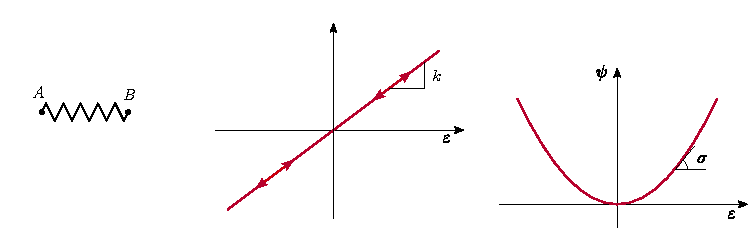
\includegraphics[scale=1.2]{figure/assunzioni_costitutive/molla}
	\caption{Materiale elastico lineare}
	\label{fig:molla}
\end{figure}

La risposta costitutiva dello sforzo: le deformazioni appaiono istantaneamente all'applicazione del carico, il legame tra lo sforzo e la deformazione è \textit{lineare} e \textit{reversibile}, nel senso che, se la forza applicata viene rimossa la deformazione è recuperata interamente:
\begin{equation}
\sigma=\widehat{\sigma}(\varepsilon)=k\,\varepsilon.
\end{equation}
La costante $k$, che fornisce la pendenza del diagramma, rappresenta la \textit{rigidezza} della molla.
L'energia è quadratica nella deformazione:
\begin{equation}
\psi=\widehat{\psi}(\varepsilon)=\frac{1}{2}k \varepsilon^2.
\end{equation}


\subsection{Materiale viscoso lineare}
Un materiale viscoso lineare obbedisce alla legge costitutiva\footnote{Si noti che la viscosità è generalmente definita in un esperimento di scorrimento, ma qui, per ragioni di convenienza notazionale, la definiamo in un processo di trazione-compressione.}
	\begin{equation}
	\sigma=\widehat{\sigma}(\dot\varepsilon)=\eta \dot{\varepsilon},
\end{equation}
dove $\eta >0$ è il coefficiente di viscosità. 



La natura costitutiva di un dispositivo reologico è spesso analizzata facendo due tipi di esperimenti: \textit{creep} e \textit{rilassamento}. L'obiettivo dell'esperimento di \textit{creep} è di misurare come un materiale si deforma nel tempo sotto un carico costante. L'obiettivo dell'esperimento di \textit{rilassamento} è di misurare come la tensione in un materiale cambia quando la deformazione è mantenuta costante.

In un esperimento di creep, quando viene applicato un carico costante, un materiale viscoso, come un fluido Newtoninao puro (ad esempio l'acqua o l'olio), inizia a deformarsi immediatamente e continua a farlo fintanto che il carico è presente; la deformazione avviene ad una velocità costante nel tempo, senza mai stabilizzarsi; questi significa che il materiale continua a ``fluire'' indefinitamente finché il carico è applicato.Non c'è una fase di deformazione elastica, poiché il materiale non immagazzina energia elastica: tutto lo sforzo applicato viene dissipato attraverso il flusso viscoso.
Il grafico della deformazione nel tempo è una linea retta, con una pendenza costante. Questa pendenza è proporzionale alla viscosità del materiale: materiali con viscosità più bassa si deformano più rapidamente.

In un materiale completamente viscoso, mantenere una deformazione costante per un esperimento di rilassamento è complicato, perché il materiale continua a deformarsi nel tempo. Tuttavia, ipotizzando un scenario ideale in cui la deformazione è istantaneamente mantenuta costante, la tensione applicata diminuisce immediatamente a zero. Questo accade perché un fluido viscoso puro non è in grado di mantenere la tensione; una volta che la deformazione è applicata, il materiale fluisce per ``alleviare'' tutta la tensione interna. Non c'è rilassamento graduale nel tempo, poiché il materiale non ha componenti elastiche per mantenere la tensione; questa  svanisce istantaneamente una volta che il moto è terminato e non rimane tensione residua nel materiale.

In Fig. \ref{fig:dashpot} è rappresentato il simbolo di uno modello reologico viscoso (uno smorzatore oleodinamico), con i grafici conseguenti ai due esperimenti descritti.
\begin{figure}[h]
	\centering
	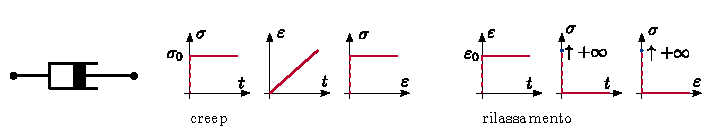
\includegraphics[scale=1.2]{figure/assunzioni_costitutive/dashpot}
	\caption{Materiale viscoso}
	\label{fig:dashpot}
\end{figure}



\subsection{Materiale plastico}
Un materiale plastico  non si deforma fino a quando lo stress  non supera una certa soglia, dopo di che scorre senza ulteriore aumento dello stress, rappresentando una deformazione plastica perfetta. Quando la forza esterna viene rimossa, la deformazione rimane in maniera permanente. 

Il comportamento del modello reologico  plastico è descritto dalle seguenti leggi:
\begin{equation}
	\begin{cases}|\sigma|\leq\bar{\sigma}\\|\dot{\varepsilon}_\mathrm{p}|\geq0\\(|\sigma|-\bar{\sigma})|\dot{\varepsilon}_\mathrm{p}|=0\end{cases}
\end{equation}
dove $\bar{\sigma}$ indica il valore della soglia di sforzo sotto la quale non vi è deformazione, mentre $\varepsilon_{\rm p}$ la deformazione plastica permanente.

Il materiale non è in grado di immagazzinare energia, ma viene totalmente dissipata.

\begin{figure}[h]
	\centering
	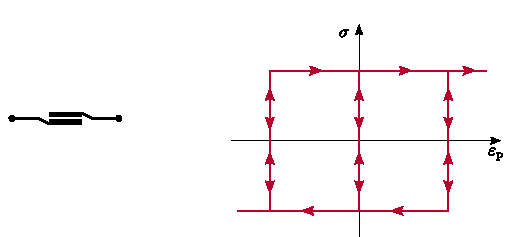
\includegraphics[scale=1.3]{figure/assunzioni_costitutive/slider}
	\caption{Materiale plastico.}
	\label{fig:slider}
\end{figure}

In Fig. \ref{fig:slider} è rappresentato il simbolo di uno modello reologico plastico (un pattino con attrito) insieme al diagramma sforzo deformazione in un ciclo completo di carico-scarico.

Il comportamento dei materiali reali non è (quasi) mai aderente ai modelli ideali appena proposti, ma spesso è descrivibile combinando i vari dispositivi proposti. Nel seguito analizziamo rapidamente alcuni modelli reologici ottenuti assemblando i dispositivi elementari elementari appena descritti.

\subsection{Materiale visco-elastico}
La combinazione di comportamenti elastici e viscosi dà luogo alla visco-elasticità, un comportamento molto comune nei materiali biologici.

È possibile assembrare molle e smorzatori in diversi modi. Consideriamo i due presentati nella Fig.  \ref{fig:MaxwellVoigt}.

\begin{figure}[h]
	\centering
	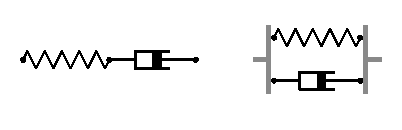
\includegraphics[scale=1.3]{figure/assunzioni_costitutive/Maxwell_Voigt}
	\caption{Materiali visco-elastici: modello di Maxwell (sinistra) e di Kelvin (destra).}
	\label{fig:MaxwellVoigt}
\end{figure}


\subsubsection{Modello di Kelvin}
Il modello di \textit{Kelvin}  è costituito da una molla e uno smorzatore collegati in parallelo. Questo modello è utilizzato per descrivere il comportamento di materiali viscoelastici solidi. Quando viene applicata una forza, la molla tenta di deformarsi istantaneamente, ma lo smorzatore resiste al movimento, causando una deformazione ritardata nel tempo. 

Lo sforzo totale di divide in una parte elastica e una viscosa:
\begin{equation}
	\sigma =\widehat{\sigma}(\varepsilon, \dot{\varepsilon})= \widehat\sigma_{\rm e}(\varepsilon)+\widehat\sigma_{\rm v}(\dot{\varepsilon}),  
\end{equation}
tali che
\begin{equation}
%\sigma=\widehat{\sigma}(\varepsilon, \dot{\varepsilon}), \qquad   
			\widehat\sigma_{\rm e}\coloneqq\widehat{\sigma}(\varepsilon,0)=k \varepsilon, \qquad \widehat\sigma_{\rm v}(\dot{\varepsilon})\coloneqq \widehat{\sigma}(\varepsilon, \dot{\varepsilon})-\widehat\sigma_{\rm e}(\varepsilon)=\eta\dot{\varepsilon}.
\end{equation}
Ne segue che, nel modello di Kelvin,
\begin{equation}
		\sigma =\widehat{\sigma}(\varepsilon, \dot{\varepsilon})=k \varepsilon+\eta\dot{\varepsilon}.
\end{equation}

Determiniamo la deformazione in un esperimento di \textit{creep}, per cui $\sigma =\sigma_0$; si tratta di risolvere l'equazione differenziale 
\begin{equation}
	k \varepsilon(t)+\eta\dot{\varepsilon}(t)=\sigma_0,
\end{equation}
la cui soluzione è
\begin{equation}
\varepsilon(t)=	\varepsilon_0+\left(\frac{\sigma_0}k-\varepsilon_0\right)\left(1-e^{-\frac k\eta t}\right).
\end{equation}
Dunque, 
in un esperimento di creep, il materiale ha un comportamento esponenziale: si deforma nel tempo fino a raggiungere un equilibrio. Lo smorzatore causa una deformazione graduale, mentre la molla impone un limite alla deformazione totale. Se all'istante $\bar{t}$ la forza viene rimossa, la deformazione decresce esponenzialmente e torna a zero, v. Fig. \eqref{fig:maxwellvoigteps}. Il modello non prevede rilassamento dello stress sotto deformazione costante $\varepsilon_0$ perché, in questo caso $\dot{\varepsilon}=0$ e dunque sforzo e deformazione sono proporzionali: $\widehat{\sigma}=k \varepsilon_0$.


\begin{figure}[h]
	\centering
	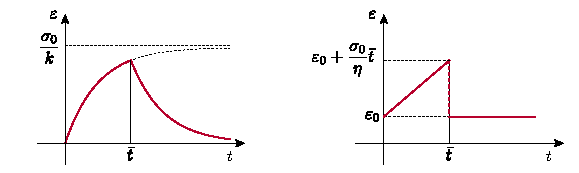
\includegraphics[scale=1.3]{figure/assunzioni_costitutive/Maxwell_Voigt_eps}
	\caption{Esperimento di creep nel modello di Kelvin (sinistra) e nel modello di Maxwell (destra).}
	\label{fig:maxwellvoigteps}
\end{figure}

Il modello di Kelvin descrive materiali viscoelastici solidi che, sotto carico costante, si deformano lentamente fino a raggiungere un equilibrio e non mostrano rilassamento dello sforzo.

%\begin{itemize}
%\item \textit{Gomma naturale}.\\
%La gomma naturale si deforma quando viene applicato un carico e lentamente raggiunge un equilibrio. Quando viene rilasciato lo stress, tende a tornare alla sua forma originale, sebbene il processo possa richiedere tempo.
%
%\item \textit{Tessuti molli biologici (come muscoli e tendini)}.\\
%Questi tessuti mostrano una deformazione lenta sotto carichi applicati, ma alla fine si stabilizzano. Questo è importante per il loro ruolo nel corpo umano, dove devono mantenere la struttura e la funzione sotto forze costanti.
%
%\item \textit{Polimeri semicristallini} (come il polietilene).\\
%Questi materiali hanno una componente elastica dovuta alla fase cristallina e una componente viscoelastica dovuta alla fase amorfa. Sotto carico, mostrano un comportamento di creep, ma raggiungono un limite.
%
%\item \textit{Leghe metalliche a bassa temperatura}.\\
%Alcune leghe metalliche possono mostrare un comportamento simile a quello del modello di Kelvin, specialmente a temperature inferiori a quelle in cui avviene un significativo scorrimento viscoso.
%\end{itemize}


\subsubsection{Modello di Maxwell}
Il modello di \textit{Maxwell} consiste in una molla e uno smorzatore collegati in serie. Questo modello è spesso usato per descrivere il comportamento viscoelastico dei fluidi e dei materiali che si comportano in modo liquido a lungo termine. Poiché i due elementi sono collegati in serie, lo sforzo $\sigma$ è lo stesso in entrambi, mentre la deformazione totale è la somma delle deformazioni della molla e dello smorzatore:
\begin{equation}
\varepsilon=\varepsilon_{\rm e}+\varepsilon_{\rm v}, \qquad \varepsilon_{\rm e}=\frac{\sigma}{k}, \quad \varepsilon_{\rm v}=\frac{1}{\eta}\int_0^t\sigma(\tau)\,\dd \tau.
\end{equation}
Derivando rispetto al tempo, si ha
\begin{equation}
\dot{\varepsilon}=\frac{\dot \sigma}{k}+\frac{\sigma}{\eta}.
\end{equation}

In un esperimento di creep viene applicato uno stress $\sigma_0$ costante; si deve allora risolvere l'equazione 
\begin{equation}
	\dot{\varepsilon}=\frac{\sigma_0}{\eta},
\end{equation}
la cui soluzione è
\begin{equation}
\varepsilon(t)=\frac{\sigma_0}{\eta}\,t+\varepsilon_0.
\end{equation}
La deformazione $\varepsilon(t)$ aumenta linearmente con il tempo; questo indica che il materiale si comporta come un fluido viscoelastico, continuando a deformarsi indefinitamente sotto carico costante. A differenza del modello di Kelvin, nel modello di Maxwell la deformazione non si stabilizza mai, ma continua ad aumentare finché lo stress è applicato.

In un esperimento di rilassamento la deformazione è costante $\varepsilon_0$, lo sforzo è risolve l'equazione differenziale
\begin{equation}
	\frac{\dot \sigma}{k}+\frac{\sigma}{\eta}=0,
\end{equation}
la cui soluzione è
\begin{equation}
	\sigma(t)=\sigma_0e^{-\frac{k}{\eta}\,t}.
\end{equation}
Lo sforzo diminuisce esponenzialmente nel tempo. Il tempo caratteristico di questo rilassamento è dato da $k/\eta$; lo sforzo nel materiale si dissipa nel tempo, il che è tipico del comportamento viscoelastico, dove l'energia immagazzinata nella molla si trasferisce allo smorzatore e si disperde come calore.

Il modello di Maxwell è applicabile a materiali viscoelastici che si comportano più come fluidi a lungo termine, mostrando creep continuo e rilassamento dello sforzo.
%
%\begin{itemize}
%\item \textit{Bitume}.\\
%Utilizzato in pavimentazioni stradali, il bitume mostra un comportamento viscoelastico fluido sotto carichi costanti, scorrendo lentamente e deformandosi permanentemente nel tempo.
%
%\item \textit{Gelatine e gel viscoelastici}.\\
%Alcuni gel, come quelli usati in alimenti o prodotti cosmetici, mostrano un comportamento viscoelastico descritto dal modello di Maxwell, con deformazione continua sotto un carico costante.
%
%\item \textit{Polimeri amorfi} (come il polistirene ad alte temperature).\\
%A temperature superiori alla transizione vetrosa, i polimeri amorfi si comportano come fluidi viscoelastici, deformandosi continuamente sotto stress.
%\end{itemize}

\begin{remark}
Ispezionare il comportamento a lungo termine dei modelli reologici fornisce un criterio di classificazione conveniente degli stati di aggregazione. Un materiale è
\begin{itemize}
	\item un \textit{solido} se in un esperimento di creep
	\begin{equation}
		\lim_{t\to\infty}\varepsilon(t)\neq 0
	\end{equation}
e in un esperimento di rilassamento
\begin{equation}
\lim_{t\to\infty}\sigma(t)\neq 0;
\end{equation}
\item un \textit{fluido} se in un esperimento di creep
\begin{equation}
	\lim_{t\to\infty}\varepsilon(t)=\infty
\end{equation}
e in un esperimento di rilassamento
\begin{equation}
	\lim_{t\to\infty}\sigma(t)= 0.
\end{equation}
\end{itemize}
Con questo criterio, un materiale elastico è un solido, mentre un materiale viscoso e di Maxwell hanno il comportamento di fluidi.
\end{remark}

%
%\begin{remark}
%Le proprietà viscoelastiche  dell'unità muscolotendinea, si manifestano nelle attività quotidiane. Ad esempio, quando una persona cerca di allungarsi per toccare le dita dei piedi, l'allungamento inizialmente è elastico. Tuttavia, man mano che l'allungamento viene mantenuto, l'ulteriore elongazione del muscolo risulta dalla viscosità della struttura muscolo-tendinea, e le dita delle mani si avvicinano lentamente al pavimento.
%
%\begin{center}
%	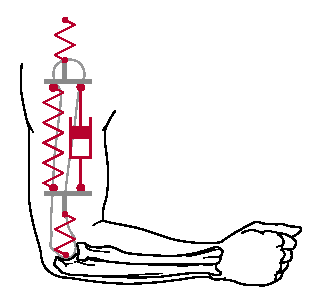
\includegraphics[width=0.6\linewidth]{figure/problema_elastico/cliniche/muscolo_visco}
%\end{center}
%
%
%L'unità muscolotendinea può essere rappresentata come composta da una componente contrattile viscosa (uno smorzatore) in parallelo con una componente elastica (una molla) e in serie con un'altra componente elastica (molla). La componente contrattile è rappresentata dalle proteine contrattili della miofibrilla, actina e miosina; i ponti trasversali della miosina possono anche mostrare una certa elasticità. La componente elastica in parallelo comprende il tessuto connettivo che circonda le fibre muscolari (l'epimisio, il perimisio e l'endomisio) e il sarcolemma. La componente elastica in serie è rappresentata dai tendini.

%\end{remark}

\subsection{Materiale elasto-plastico}
\subsubsection{Materiale elastico perfettamente plastico}
Un dispositivo reologico composto da una molla lineare e un pattino con attrito collegati in serie descrive un  comportamento che combina i caratteri dei materiali elastici e perfettamente plastici. Questo sistema può essere utilizzato per modellare materiali che mostrano un comportamento elastico fino a un certo punto e, oltre tale punto, una deformazione permanente.

\begin{figure}[h]
	\centering
	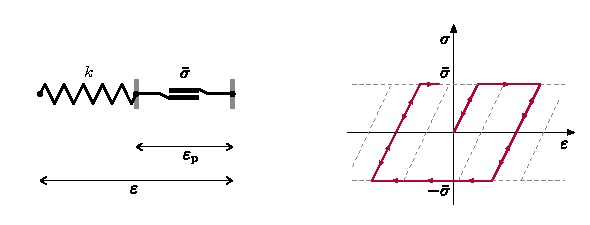
\includegraphics[scale=1.3]{figure/assunzioni_costitutive/elastoplastico}
	\caption{Materiale elastico perfettamente plastico.}
	\label{fig:elastoplastico}
\end{figure}


Quando si applica una forza esterna al sistema, cui corrisponde uno sforzo $\sigma$, la molla si deforma elasticamente secondo la relazione $\sigma=k \varepsilon$. Se lo sforzo  è inferiore a $\bar\sigma$, viene interamente sostenuto dalla molla, e il pattino rimane fermo; la deformazione totale del sistema è puramente elastica e data da $\varepsilon=\sigma/k$. In questa fase, il comportamento del sistema è elastico lineare.

Quando lo sforzo raggiunge il valore limite $\bar{\sigma}$ (detto di snervamento), il pattino inizia a scivolare. In questo momento, la molla continua a fornire una resistenza elastica, ma il sistema può ora sostenere un incremento di deformazione senza un ulteriore incremento di sforzo. Dopo lo snervamento, lo sforzo  rimane costante a $\bar\sigma$; la deformazione totale è composta dalla deformazione elastica (limitata dalla molla) e da una deformazione plastica che cresce indefinitamente:
\begin{equation}
	\varepsilon=\frac{\sigma}{k}+\varepsilon_{\rm p},
\end{equation}
Dove $\varepsilon_{\rm p}$ è la deformazione plastica, che continua ad aumentare senza limiti finché il pattino continua a scorrere.

Quando si riduce lo stress, la deformazione elastica si recupera. Il diagramma sforzo deformazione segue una linea retta con la stessa pendenza della fase di carico elastico. Tuttavia, poiché c'è stata una deformazione plastica permanente durante il carico, il diagramma non torna all'origine ma a una deformazione residua, che rappresenta la parte permanente della deformazione plastica. La tensione vale
\begin{equation}
	\sigma=k(\varepsilon-\varepsilon_{\rm p}).
\end{equation}
Quando lo sforzo è ridotto a zero, la deformazione elastica è completamente recuperata, ma la deformazione residua rimane. Se si continua a scaricare, si raggiunge la soglia $-\bar{\sigma}$, oltre la quale lo sforzo continua a rimanere costante. Se si carica nuovamente, il diagramma segue inizialmente la stessa linea retta, fino a raggiungere nuovamente lo sforzo di snervamento.

Il diagramma (v. Fig. \ref{fig:elastoplastico}) presenta un ciclo di \textit{isteresi}, un fenomeno in cui la risposta del materiale  a un cambiamento dello sforzo dipende dalla storia passata di quella variabile. Questo significa che la relazione tra  sforzo e deformazione non segue lo stesso percorso durante l'incremento e il decremento della variabile. In un materiale che mostra isteresi, parte dell'energia meccanica immagazzinata durante la fase di carico non viene completamente restituita durante la fase di scarico. Questa perdita di energia è tipica di materiali plastici e rappresenta la dissipazione interna dovuta a fenomeni come attrito interno e scorrimento.

\subsubsection{Materiale elasto-plastico con incrudimento}
Il modello reologico di plasticità con \textit{incrudimento} (\textit{hardening}) è una rappresentazione che descrive il comportamento di materiali che non solo si deformano plasticamente dopo il superamento di un certo limite di snervamento, ma che diventano progressivamente più resistenti (cioè ``induriti'') man mano che la deformazione plastica procede. Questo modello è particolarmente utile per descrivere materiali metallici che, dopo il superamento del limite elastico, richiedono un aumento dello sforzo per continuare a deformarsi plasticamente.


Un modello reologico che descrive la plasticità con incrudimento può essere rappresentato utilizzando una combinazione di elementi semplici: 1) Molla lineare di rigidezza $k$ in parallelo: rappresenta il comportamento elastico del materiale; pattino con attrito in serie a una molla  lineare di rigidezza $h$: rappresenta la plasticità e l'incrudimento. Il pattino con attrito descrive la fase in cui il materiale scorre plasticamente, mentre la molla  lineare rappresenta l'incremento di resistenza del materiale man mano che la deformazione plastica procede.

\begin{figure}[h]
	\centering
	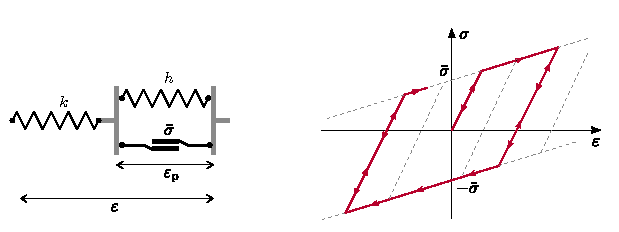
\includegraphics[scale=1.3]{figure/assunzioni_costitutive/hardening}
	\caption{Materiale elasto-plastico con incrudimento.}
	\label{fig:hardening}
\end{figure}

All'inizio, il carico applicato deforma elasticamente il sistema fino al punto di snervamento $\bar{\sigma}$; la relazione costitutiva è data da $\sigma=k\varepsilon$. Quando  lo sforzo raggiunge $\bar{\sigma}$, il pattino inizia a muoversi, segnalando l'inizio della deformazione plastica. A questo punto, la molla lineare aggiunta in serie comincia a deformarsi, inducendo un incrudimento lineare.

Dopo lo snervamento, l'aumento di sforzo richiesto per ulteriori deformazioni è proporzionale alla deformazione plastica accumulata; la nuova relazione tra sforzo e deformazione è $\sigma=\bar{\sigma}+h\varepsilon_{\rm p}$
dove $h$  è il modulo di incrudimento e $\varepsilon_{\rm p}$ la deformazione plastica: per ogni incremento di deformazione plastica, lo sforzo aumenta linearmente. 

Il modello si applica a molti materiali di largo uso in svariati contesti come ad esempio gli acciai.
%\begin{itemize}
%	\item \textit{Acciai ad alto tenore di carbonio}.\\
%	Questi materiali spesso mostrano un incrudimento lineare oltre il limite di snervamento, utile per applicazioni strutturali.
%	\item \textit{Polimeri Ingegneristici}.\\
%	Alcuni polimeri, come il policarbonato e il nylon, presentano un comportamento plastico con incrudimento lineare quando sono soggetti a carichi elevati.  Il policarbonato è utilizzato in applicazioni che richiedono trasparenza e resistenza meccanica, come lenti protettive e parti di macchine. Il nylon, per esempio, è impiegato per fibre tessili, dove è importante che il materiale resista alla deformazione durante l'uso senza perdere le sue proprietà meccaniche.
%	\item \textit{Leghe di Titanio}.\\
%	Le leghe di titanio, note per la loro elevata resistenza e bassa densità, mostrano un comportamento plastico con incrudimento lineare. Questo le rende particolarmente adatte per applicazioni dove il peso deve essere minimizzato senza compromettere la resistenza. Le leghe di titanio sono usate per protesi, dove è essenziale che il materiale possa resistere a deformazioni durante l'impianto e l'uso quotidiano; la capacità di indurirsi sotto carico permette alla protesi di essere duratura e resistente, riducendo il rischio di fallimento meccanico e la necessità di revisioni chirurgiche.
%\end{itemize}


%\subsection{Materiali visco-elasto-plastici}


%
%\newpage
%\section{Materiali elasto-plastici}
%In fig. \eqref{fig:acciaio} è riportata la curva caratteristica della risposta costitutiva della tensione  rispetto alla deformazione () e l'andamento del rapporto tra la contrazione trasversale e l'allungamento assiale di un provino d'acciaio
%
%\begin{figure}
%	\centering
%	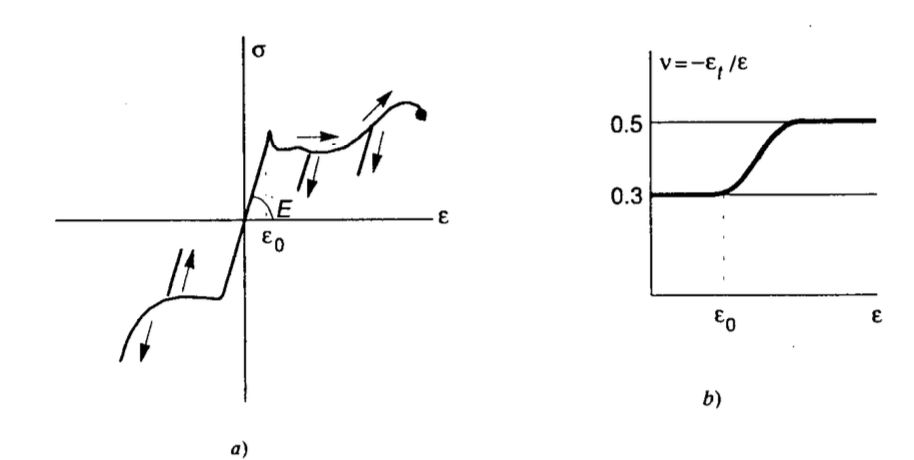
\includegraphics[width=0.7\linewidth]{figure/assunzioni_costitutive/acciaio}
%	\caption{Prova di trazione per un acciaio.}
%	\label{fig:acciaio}
%\end{figure}
%
%Notiamo alcuni aspetti caratteristici:
%\begin{enumerate}
%\item Le deformazioni appaiono istantaneamente all'applicazione del carico.
%\item In una prima fase, il legame tra la tensione e la deformazione è \textit{lineare} e \textit{reversibile}, nel senso che, se la forza applicata viene rimossa la deformazione è recuperata interamente. Questa fase termina quando la deformazione raggiunge un certo valore limite $\varepsilon_0$, cui corrisponde uno sforzo $\sigma_0$.
%\item Per $\varepsilon>\varepsilon_0$ il comportamento è sensibilmente differente. Innanzitutto, a un dato incremento di deformazione corrisponde un incremento di sforzo molto minore di prima; addirittura in una prima fase pressoché nullo: il materiale scorre come se fosse  un fluido. Inoltre le deformazioni diventano \textit{permanenti}, in quanto allo scarico solo una parte viene recuperate. In questa fase il materiale ha un comportamento \textit{plastico}.
%\item Il provino, allungandosi si contrae trasversalmente. Il rapporto tra i valori assoluti della deformazione  trasversale e assiale tende rapidamente a 1/2.
%\end{enumerate}
%
%Questi aspetti fenomenologici devono essere inclusi nel modello costitutivo. 
%
%
%
%
%\begin{figure}
%	\centering
%	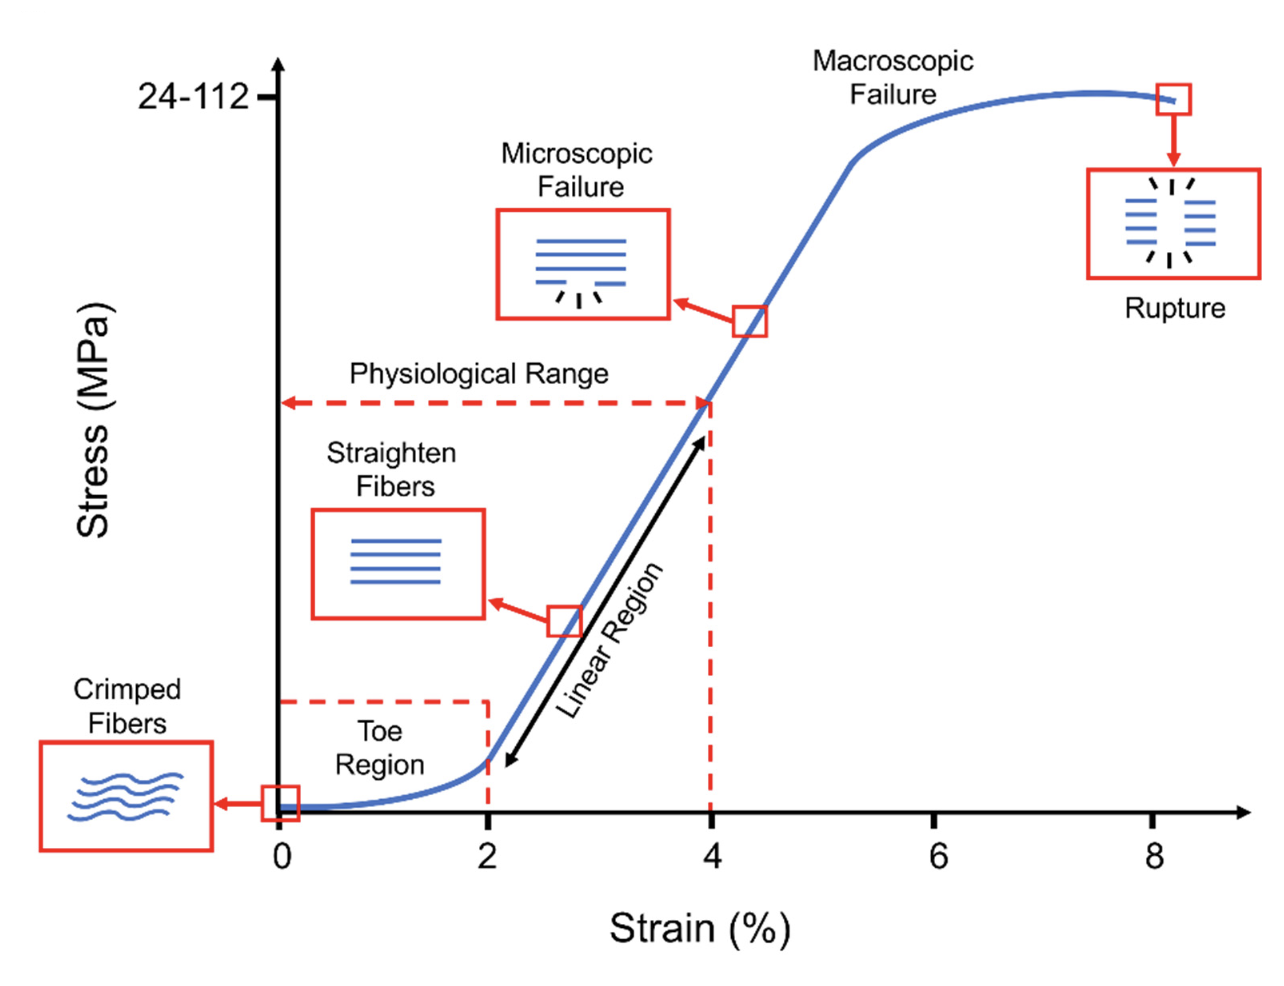
\includegraphics[width=0.7\linewidth]{figure/assunzioni_costitutive/ligament}
%	\caption{Legame sforzo-deformazione per un tendine}
%	\label{fig:ligament}
%\end{figure}
%
%\newpage
%\begin{figure}
%	\centering
%	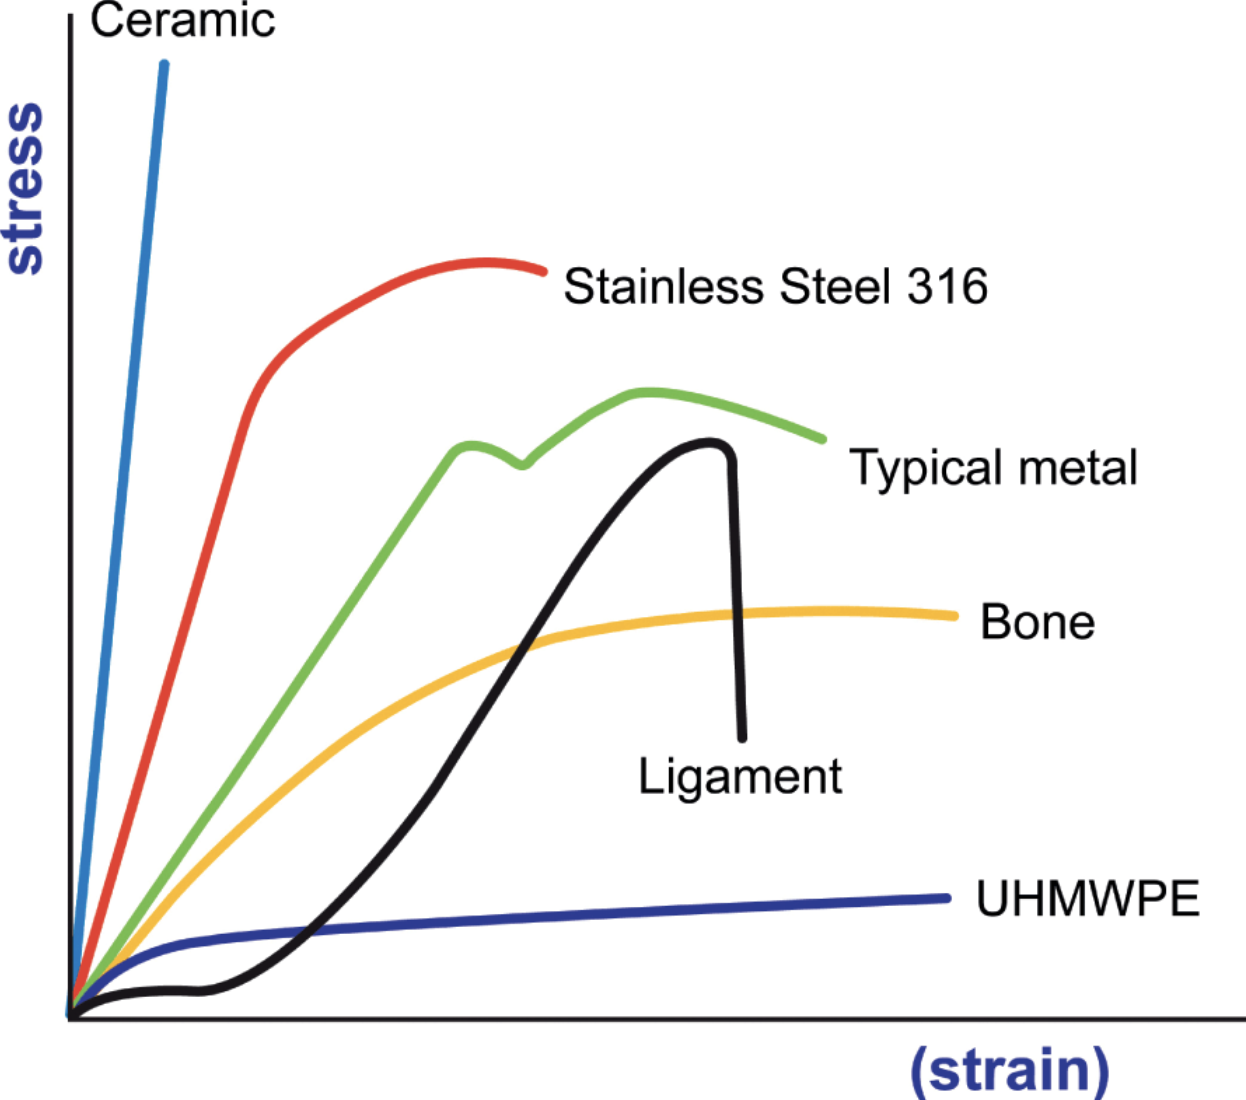
\includegraphics[width=0.5\linewidth]{figure/assunzioni_costitutive/stressstrain}
%	\caption{Legame sforzo-deformazione per differenti materiali di interesse biomedico.}
%	\label{fig:stressstrain}
%\end{figure}
